% Chapter 2

\chapter{Simulating Orbits} % Main chapter title

\label{Chapter2} % For referencing the chapter elsewhere, use \ref{Chapter1} 

\lhead{Chapter 2. \emph{Simulating Orbits}} % This is for the header on each page - perhaps a shortened title

%----------------------------------------------------------------------------------------

In this chapter, a more advanced simulation of orbiting masses will be introduced.  First, a simple orbit situation will be introduced, followed by more complex examples involving escape velocities.  Finally, Kepler's 2nd law will be examined from a simulation of an orbiting planet.


\section{Basic Orbit Path}

The first simulation will deal with an example of a planet orbiting another much more massive planet.  

\subsection{Background Physics}



This entire chapter is centered around Newton's law of universal gravitation:

\begin{equation}\label{universalgravity}
F_g = G \frac{m_1 m_2}{r^2} 
\end{equation}

Where $F_g$ is the magnitude of the force acting on either mass, G is the gravitational constant ( SI units of $6.67 \hspace{1mm} \frac{Nm^2}{kg^2}$ ), $m_1$ is the mass of one object, $m_2$ is the mass of the other object, and $r$ is the radius separating the two masses.  By Newton's 3rd law, there is an equal and opposite force exerted on each mass.  

This equation can be used to describe the orbiting paths of planets.  For simple cases when one planet orbits another, the variables m and M can be used.  For a first example, we will assume M \textgreater \textgreater  m, that is, one planet has a much greater mass than the other.  Therefore, while each planet exerts an equal force on the other, the acceleration on the massive planet will be negligible.  So, the smaller planet will orbit around the stationary planet, without attracting the larger planet enough to move it.  




\subsection{The Code}  

The full code is shown in the listing below:

\setstretch{1}
\begin{lstlisting}[breaklines=true, frame=single, numbers=left, caption=Basic planet orbiting simulation, label=lst:basicorbit]
var canvas = document.getElementById('canvas');
var context = canvas.getContext('2d'); 
var canvas_bg = document.getElementById('canvas_bg');
var context_bg = canvas_bg.getContext('2d');

var planet;
var sun;
var m = 1; // planet's mass
var M = 1000000; // heavy planet's mass
var G = 1;
var t0,dt;

window.onload = init; 

function init() {
	// create a stationary large planet
	sun = new Ball(70,'orange',M);
	sun.pos2D = new Vector2D(275,200);	
	sun.draw(context_bg);
	// create a moving planet			
	planet = new Ball(10,'blue',m);
	planet.pos2D = new Vector2D(200,50);
	planet.draw(context);
	// make the planet orbit the large planet
	t0 = new Date().getTime(); 
	animFrame();
};

function animFrame(){
	animId = requestAnimationFrame(animFrame,canvas);
	onTimer(); 
}
function onTimer(){
	var t1 = new Date().getTime(); 
	dt = 0.001*(t1-t0); 
	t0 = t1;	
	if (dt>0.1) {dt=0;};	
	move();
}
function move(){			
	moveObject(planet);
	calcForce();
	updateAccel();
	updateVelo(planet);
}

function moveObject(obj){
	obj.pos2D = obj.pos2D.addScaled(obj.velo2D,dt);	
	context.clearRect(0, 0, canvas.width, canvas.height);
	obj.draw(context);	
}
function calcForce(){
	force = Forces.gravity(G,M,m,planet.pos2D.subtract(sun.pos2D));	
}	
function updateAccel(){
	acc = force.multiply(1/m);
}	
function updateVelo(obj){
	obj.velo2D = obj.velo2D.addScaled(acc,dt);				
}
\end{lstlisting}
\setstretch{2}

This program differs from previous ones used so far in that it uses two canvases instead of one.  This is essential for having the large planet remain stationary and not being erased every frame.  Instead, there can be a constant ``background'' canvas containing the stationary planet.  The code begins by initializing the variables planet and sun, where sun simply refers to any large planet that has much more mass.  The gravitational constant $G$ is intialized as a formality just to a value of 1.  G in this simulation isn't necessary, because the constant simply is used for unit conversion.  This will become clear later in this section.  When the web page is loaded, it calls the init function, just as in previous simulations.  The init function creates the sun and planet as objects from the Ball constructor function, exactly as in chapter 1.  Instead of having separate variables x and y in the previous examples, the position information can be stored into a property of each object, which is created using a different constructor function Vector2D.  

The next function, animFrame, functions simply by initializing the javascript animation frame, and then calling the next function, onTimer.  This next function creates a variable dt by converting the unit javascript operates in (ms) to SI units of s.  It then passes the flow of the program onto the next function, move.  This function involves calling 4 functions, the first of which simply updates the position of the planet, erases the foreground canvas, and then draws the updated canvas.  This step can be analyzed through a physics kinematics equation:

\begin{equation}\label{velo}
x(t+dt) = x(t) + v_x(t)dt
\end{equation}

This is essentially analagous to Euler's method, by understanding that $v_x = \frac{dx}{dt}$.  

\begin{equation}\label{euler}
x(t+dt) = x(t) + \frac{dx}{dt}\left(0\right) dt
\end{equation}

By using constructor functions, with 2 different properties for the x and y position, the planet's location can be updated without updating variables and taking up more space.  The location has to be updated for every frame, but so does the force, acceleration, and velocity.  These next 3 steps are the remaining functions of the move function.  The calcForce function updates the force of gravity acting on the planet, using equation \ref{universalgravity}.  This equation calculates r by calculating the displacement vector between the two planets, and finding the magnitude of that vector.  The updateAccel function simply takes the updated force vector and scales it by a certain ``k'' value which is represented by dividing by the mass.  This is the step that incorporates Newton's 2nd law of $a = \frac{F}{m} $.  The last function updates the velocity of the planet, similar to how the position was updated.  Using Euler's method like before, we come to the following equation

\begin{equation}\label{euleraccel}
 v (t+dt) =  v(t) + a(t)dt 
\end{equation}





Essentially, what makes this program more complicated is that it uses many other functions to accomplish the overall simulation.  However, this method of programming makes future simulations easier--the same functions can be used, with changed variables.  The code listing below shows these ``tool'' functions that are used in future chapters of this thesis:

\setstretch{1}
\begin{lstlisting}[breaklines=true, frame=single, numbers=left, caption=Various tools functions used for orbit simulation, label=lst:basicorbittools]
function Vector2D(x,y) {
	this.x = x;
	this.y = y;		
}	
Vector2D.prototype = {		
	lengthSquared: function(){
		return this.x*this.x + this.y*this.y;
	},
	length: function(){
		return Math.sqrt(this.lengthSquared());
	},
	add: function(vec) {
		return new Vector2D(this.x + vec.x,this.y + vec.y);
	},
	subtract: function(vec) {
		return new Vector2D(this.x - vec.x,this.y - vec.y);
	},
	multiply: function(k) {
		return new Vector2D(k*this.x,k*this.y);
	},
	addScaled: function(vec,k) {
		return new Vector2D(this.x + k*vec.x, this.y + k*vec.y);
	},	

	function Forces(){
}
Forces.gravity = function(G,m1,m2,r){
	return r.multiply(-G*m1*m2/(r.lengthSquared()*r.length()));
}
\end{lstlisting}
\setstretch{2}


\section{Escape Velocity}

The previous section tested situations where the planet orbited the sun continuously.  However, if the speed is great enough, the orbiting body is capable of ``escaping'' from the larger planet's influence.  The minimum speed necessary for this is called the escape velocity.  

This can be derived by understanding conversation of energy.  When an object leaves the surface of a planet, it will have an initial kinetic energy, and potential gravitational energy.  This will equal the final condition, when the final kinetic and gravitational potential energy is 0.\textsuperscript{\cite{engineering}}  This relationship is shown in the equation below:

$$K_i + U_{g_{i}} = K_f + U_{g_{f}}$$

Knowing that the final kinetic and gravitational energy is 0, this equation becomes:

$$\frac{1}{2}mv_{esc}^2 - \frac{GMm}{r} = 0 + 0  $$

Solving for $v_{esc}$ yields the following:

\begin{equation}\label{eq:escapevelocity}
v_{esc} = \sqrt{\frac{2GM}{r}}
\end{equation}

Where G is the gravitational constant, M is the mass of the planet the object is escaping from, and r is the starting distance from the center of mass of the planet.\textsuperscript{\cite{klepner}}  

To test the physics behind the escape velocity, a slightly different scenario can be created with a different program.  This simulation will have the object begin right at the surface of the larger planet, to emulate the process of ``escaping'' from the planet's gravity influence.  To visualize this, a much larger canvas will be used, and some code changes will be utilized, seen below:


\setstretch{1}
\begin{lstlisting}[breaklines=true, frame=single, numbers=left, caption=New conditions for escape velocity simulation, label=lst:changestoorbit]
sun = new Ball(400,'orange',M);
sun.pos2D = new Vector2D(

planet = new Ball(10,'blue',m);
planet.pos2D = new Vector2D(500,2490);

planet.velo2D = new Vector2D(0, -80);
\end{lstlisting}
\setstretch{2}

These changes made the larger planet look visually bigger, to simulate the effect of a massive planet.  It also positioned the object to begin right on the surface of the larger planet (in this case, 410 pixels above the center of mass of the larger planet).  To calculate the escape velocity for the situation above, equation \ref{eq:escapevelocity} can be used, but understanding some key factors:

\begin{enumerate}
\item The escape velocity calculated will be in $\frac{px}{s}$ instead of SI unit $\frac{m}{s}$
\item The masses of each planet don't need to contain units, it can more just represent a ratio between the large and small planet.  Therefore, each mass will be a unitless quantity, just used as a test of the escape velocity equation.
\item Similarly to  \#2, the gravitational constant G doesn't have to include units, since this test is only in a more theoretical sense, and doesn't use actual units of mass.  However, using dimensional analysis, for the equation below to make sense, G could be viewed as having units of $\frac{px^3}{s^2}$.
\end{enumerate}

Proceeding with these conditions in mind, the escape velocity for the simulation of code listing \ref{lst:changestoorbit}
can be calculated as shown below:

\begin{equation}\label{eq:calcvescape}
 v_{esc} = \sqrt{\frac{2*1 \frac{px^3}{s^2}*1000000}{410 px}} \approx 69.843 \frac{px}{s} 
\end{equation}

Therefore, with the program simulation, any initial speed greater than this value will escape the gravitational influence of the larger planet.  To test this, I used the following code to print out values of the velocity continuously:

\setstretch{1}
\begin{lstlisting}[breaklines=true, frame=single, numbers=left, caption=Code for printing out values of speed, label=lst:changestoorbit]
var i =0;
i++;
if(i%15 ===0){console.log(planet.velo2D.length());}
\end{lstlisting}
\setstretch{2}

This code operates by printing out the value of the speed of object 4 times per second, understanding that i is incremented by 1 for each frame, and there are the usual 60 frames per second.  The data is outputted through the console.log() method, which prints it onto the web browser.  This data was then plotted for different initial speeds, and the results are shown in Figures 2.1-2.3.


\begin{figure}[h] 
	\centering
		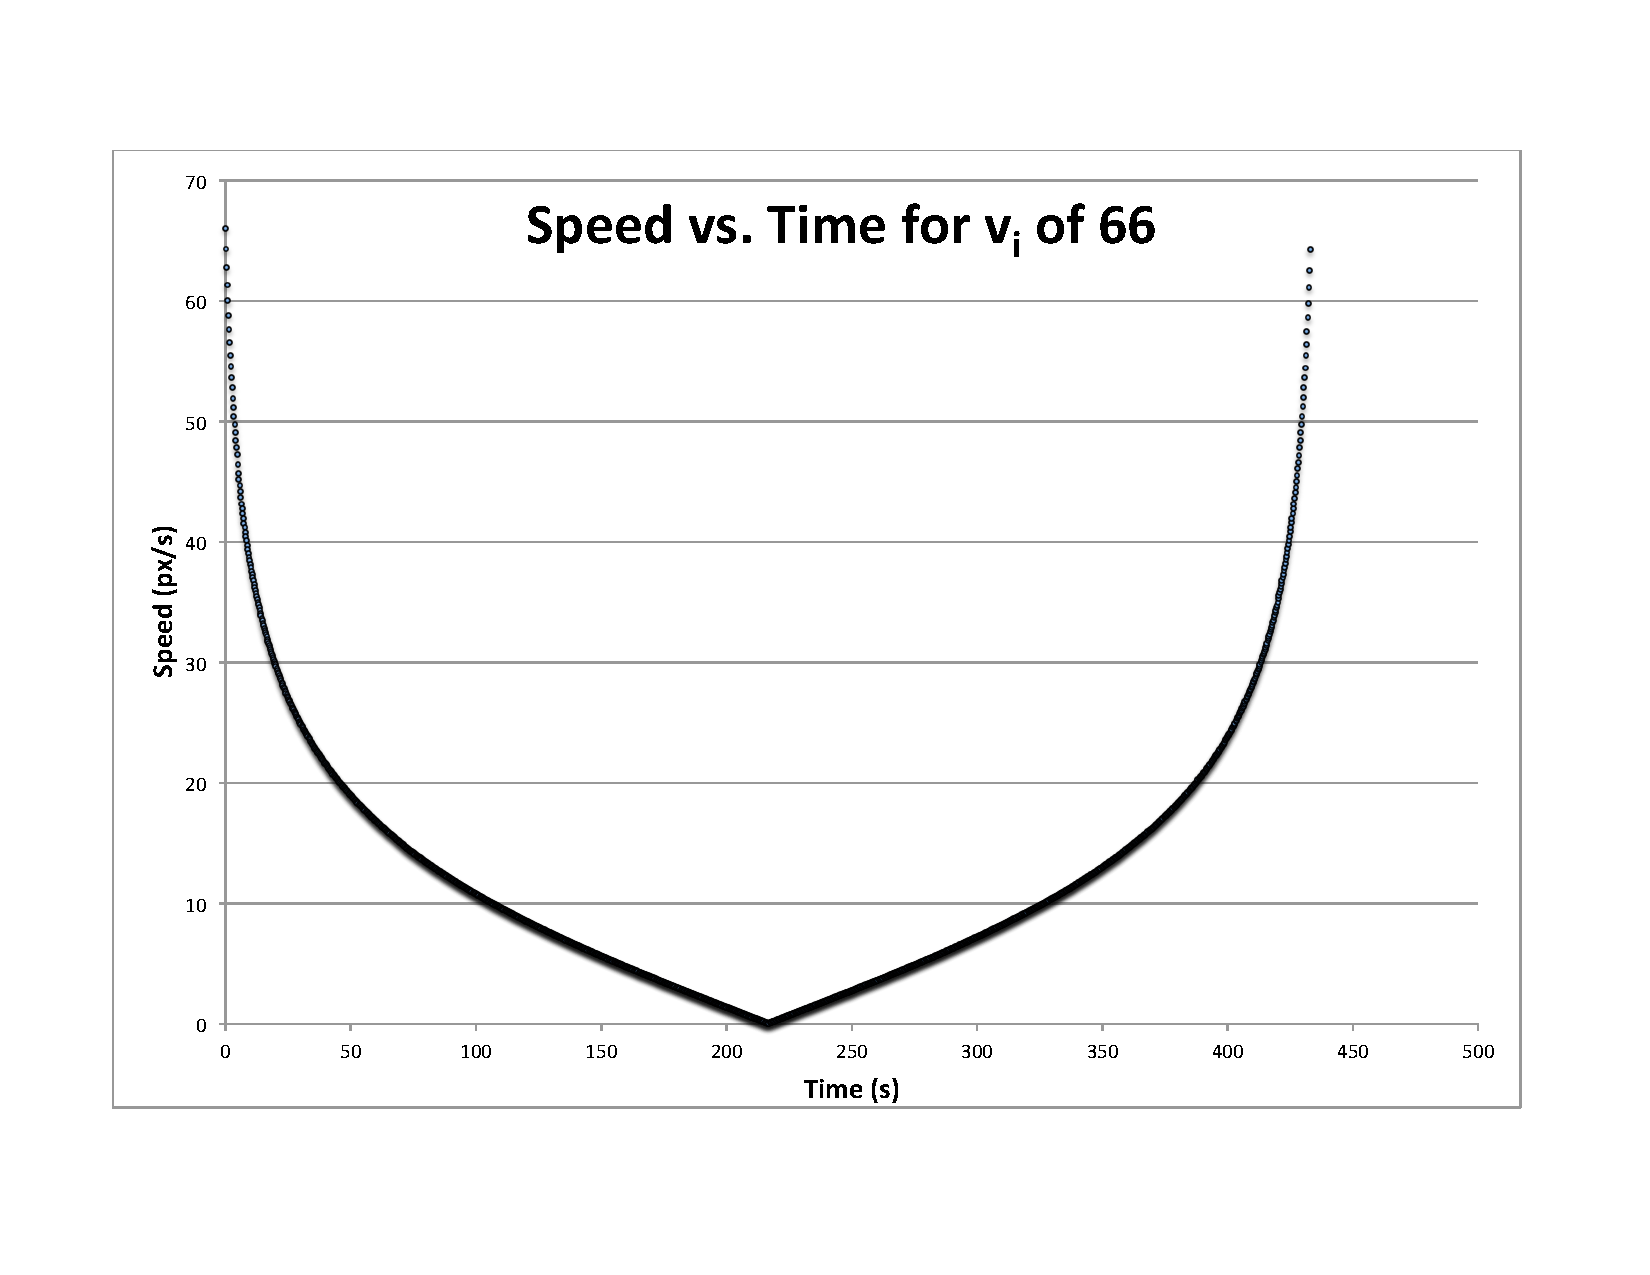
\includegraphics[width=12cm]{Figures/fig1.pdf}

	\caption{Speed vs. time for initial $v_i$ of 66 $\frac{px}{s}$}
	\label{fig:data1}
\end{figure}


\begin{figure}[h] 
	\centering
		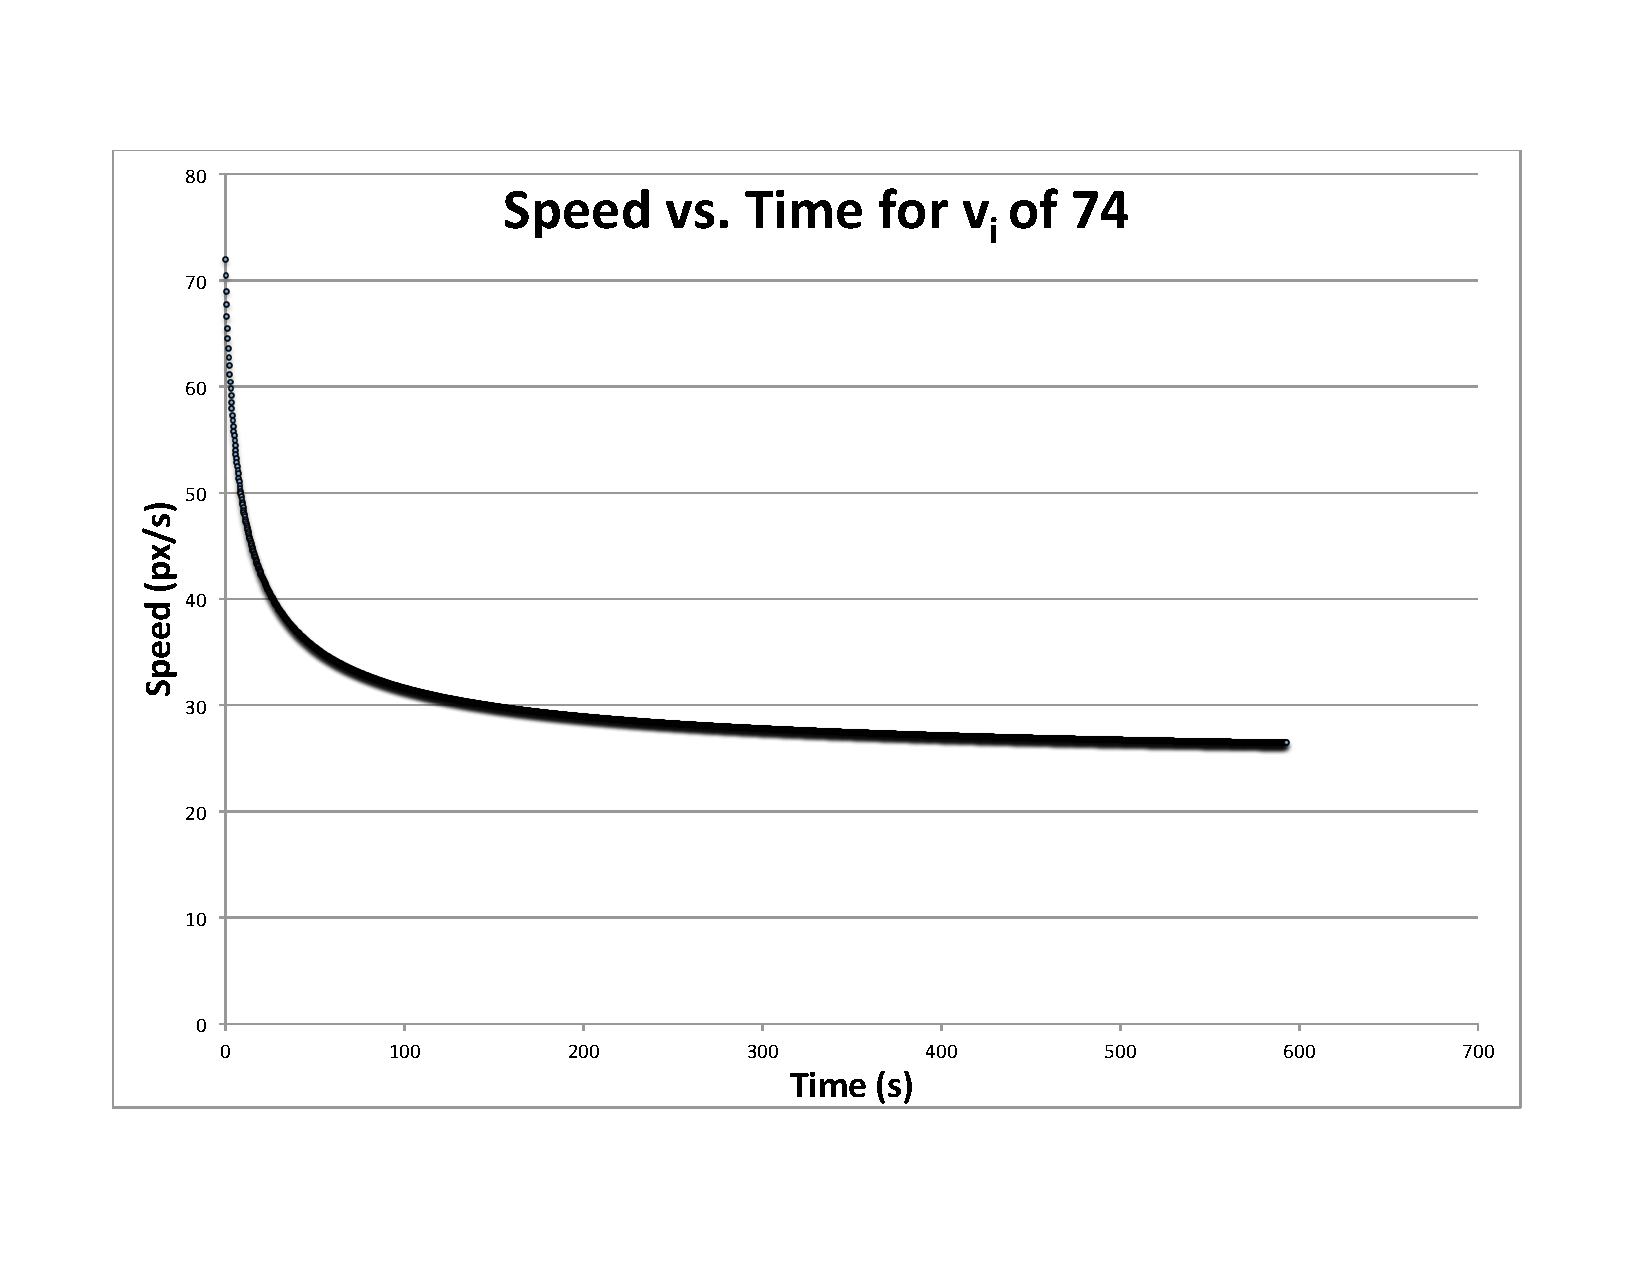
\includegraphics[width=12cm]{Figures/fig2.pdf}

	\caption{Speed vs. time for initial $v_i$ of 74 $\frac{px}{s}$}
	\label{fig:data2}
\end{figure}


\begin{figure}[h] 
	\centering
		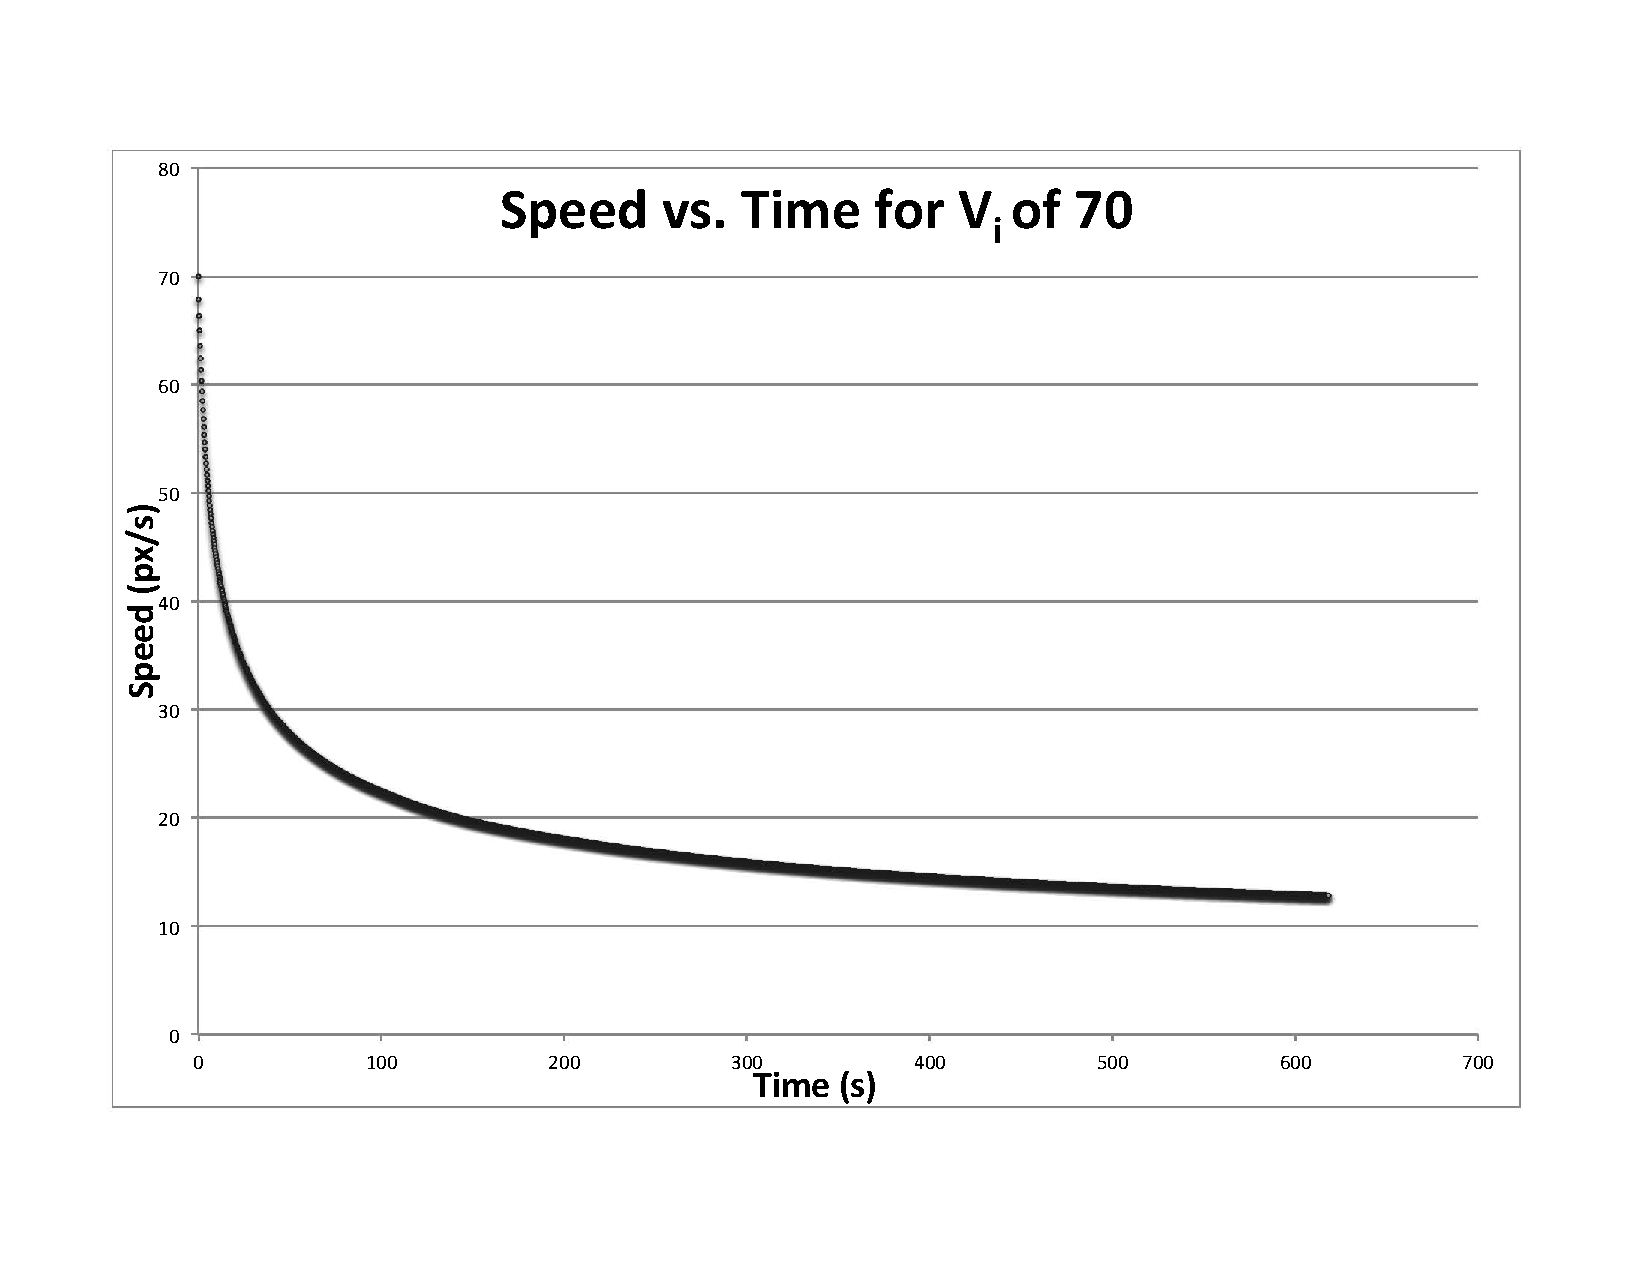
\includegraphics[width=12cm]{Figures/fig3.pdf}

	\caption{Speed vs. time for initial $v_i$ of 70 $\frac{px}{s}$}
	\label{fig:data3}
\end{figure}




These 3 figures show the speed vs. time for different intial velocities.  Figure \ref{fig:data1} shows an initial speed of 66, which isn't enough for the required 69.843 speed to leave the influence of the larger planet.  The object rises far away from the planet, slows down, and then reaches a point where the speed is 0, and then reverse direction and accelerates back towards the planet.  Figures \ref{fig:data2} and \ref{fig:data3} show initial speeds greater than that of the escape velocity, and the effect is clear: the speed tapers off eventually to an end velocity, as r approaches $\infty$ and the gravity force approaches 0.  If the initial speed exactly equaled the escape velocity, in theory the final speed of the object would approach 0, and r approaches $\infty$.  However, this simulation would take a very long time to do.  All of these graphs were plotted over times ranging from 400 to 700 seconds, and since the speed was printed 4 times per second by the computer program, there were thousands of data points plotted overall. 





\section{Kepler's Laws}




In the early 1600's Johannes Kepler proposed a series of laws that explained how planets orbit the sun.\textsuperscript{\cite{klepner}}  This was in support of the scientific-based heliocentric model, which conflicted with the geocentric model before that.  These 3 laws are shown below:



\begin{enumerate}
\item All planets move in ellpitical orbits with the Sun at one focus
\item The radius vector drawn from the Sun to a planet sweeps out equal areas in equal time intervals
\item The square of the orbital period of any planet is proportional to the cube of the semimajor axis of the elliptical orbit
\end{enumerate}

The simulation in this section will help visualize law \#2, using the orbit program already created in section 2.1  This law can be derived by understanding the situation of a planet orbiting the sun in an ellpitical.  The sun is assumed to be much more massive so it doesn't move.  At any instant along the path of orbit, the planet has a gravitational force pointing towards the sun, and it's velocity is tangential to this inward force.  This can be visualized in figure \ref{fig:sun1}.  

\begin{figure}[h] 
	\centering
		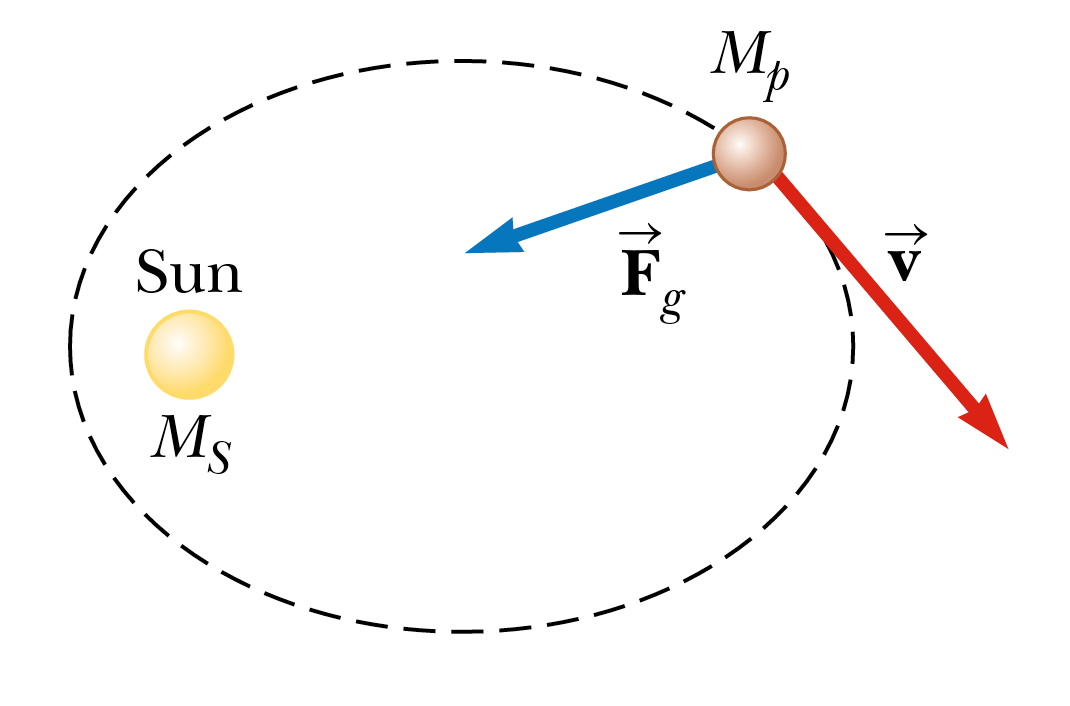
\includegraphics[width=8cm]{Figures/sun1.png}
	\caption{Basic model of planet orbiting a sun}
	\label{fig:sun1}
\end{figure}


The gravitational force is a central force that always points antiparallet to the radius vector $\vec{r}$.  Knowing the radius vector and force on the planet at any point, the torque can be calculated, from the equation below:

\begin{equation}\label{eq:torque}
\vec{\tau} = \vec{r}\times\vec{F_g} = \frac{d\vec{L}}{dt}
\end{equation}


Because the radius and force vector are always antiparallel to one another, the torque, and therefore, the change in angular momentum will equal 0.  In other words, $\vec{L}$ will remain constant.  Knowing that $\vec{p} = M_p \times \vec{v}$, the following can be derived:

$$ \vec{L} = \vec{r}\times \vec{P} = M_p \vec{r}\times\vec{v}  $$

However, since the angle between $\vec{r}$ and $\vec{v}$ is always 90\textdegree, the equation above can expressed as:


\begin{equation}\label{eq:torquederive}
L = M_p \left|\vec{r} \times \vec{v}\right|
\end{equation}

This equation can be related to figure \ref{fig:sun2}, which shows the relationship between $\vec{r}$ and $d\vec{r}$.

\begin{figure}[h] 
	\centering
		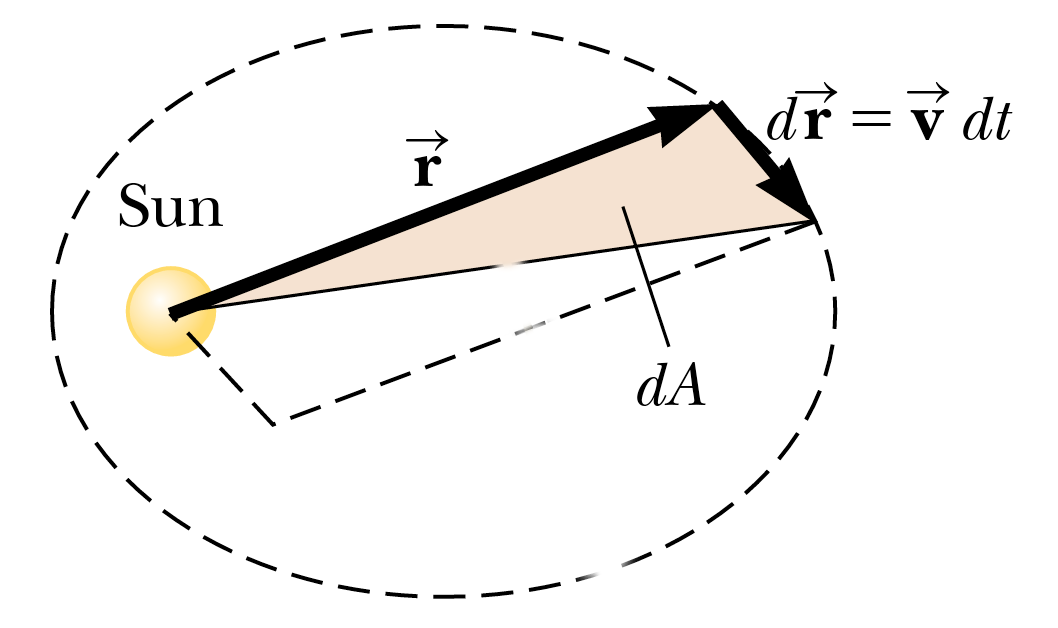
\includegraphics[width=8cm]{Figures/sun2.png}
	\caption{Relationship between  $\vec{r}$ and $d\vec{r}$}
	\label{fig:sun2}
\end{figure}

$\vec{r} \times d\vec{r}$ equals the area of the parallelogram in figure \ref{fig:sun2}.  As $dt \rightarrow  0$, the area $dA$ equals $\frac{1}{2}$ the area of this same parallelogram.\textsuperscript{\cite{klepner}}  Using this relationships yields the following:

$$ dA = \frac{1}{2}|\vec{r} \times d\vec{r}| = \frac{1}{2}\left|\vec{r} \times \vec{v} dt \right| = \frac{1}{2}\left|\vec{r} \times \vec{v}\right| dt  $$

Rearranging equation  to solve for $\left|\vec{r} \times \vec{v}\right|$, and substituting this into the above expression yields the following:

$$ dA = \frac{1}{2}\left(\frac{L}{M_p}\right)dt  $$

Finally, dividing both sides by dt yields the final equation:

\begin{equation}\label{dadt}
\frac{dA}{dt} = \frac{1}{2}\left(\frac{L}{M_p}\right)
\end{equation}

Since $L$ and $M_p$ are constants, this equation shows that the rate of change in area is constant.  To visualize this, slight adjustments were made to the simulation of section 1.  The code changes are shown below:



\setstretch{1}
\begin{lstlisting}[breaklines=true, frame=single, numbers=left, caption=Code for printing out values of speed, label=lst:changestoorbit]
if(i<960){
	if(i%30===0){
	context.strokeStyle = 'white';
	context.moveTo(planet.x, planet.y);
	context.lineTo(sun.x, sun.y);
	context.stroke();
	var dr = Vector2D.distance(planet.pos2D, planet.oldpos2D);
	var r =  Vector2D.distance(planet.pos2D, sun.pos2D);
	console.log('dA is equal to:  %f', .5*r*dr);
	planet.oldpos2D=planet.pos2D;
	}
\end{lstlisting}
\setstretch{2}

This code creates a condition where ever .5 seconds, a line is drawn between the position of the sun and the position of the planet.  This visualizes the display of breaking up the orbit path into different area segments, which should all be equal area.  Because the simulation occurs at a consistent rate of 60 frames per second, the lines could be drawn at a consistent rate over time.  The code also calculates a variable r, which is the magnitude of the displacement vector between the two positional vectors of the planet and sun.  The vector dr is also calculated by comparing the positional vectors of the planet between two different times.  With these two variables, the program performs a rough calculation of dA, by understanding it is approximately $\frac{1}{2}$ the area of the parallelogram.  The areas were the same within a reasonable amount of uncertainty and accuracy possible with the javascript program.  The smallest ``dt'' possible in this program is 17 ms due to the limitations of the animation method of javascript.  However, if dt could be made to approach 0, the calculations of dA would likely be closer to one another.

A screenshot of the simulation is shown in figure \ref{fig:screenshot}.  This helps to visually understand Kepler's 2nd law by separating areas of the same change in time by lines.

\begin{figure}[h] 
	\centering
		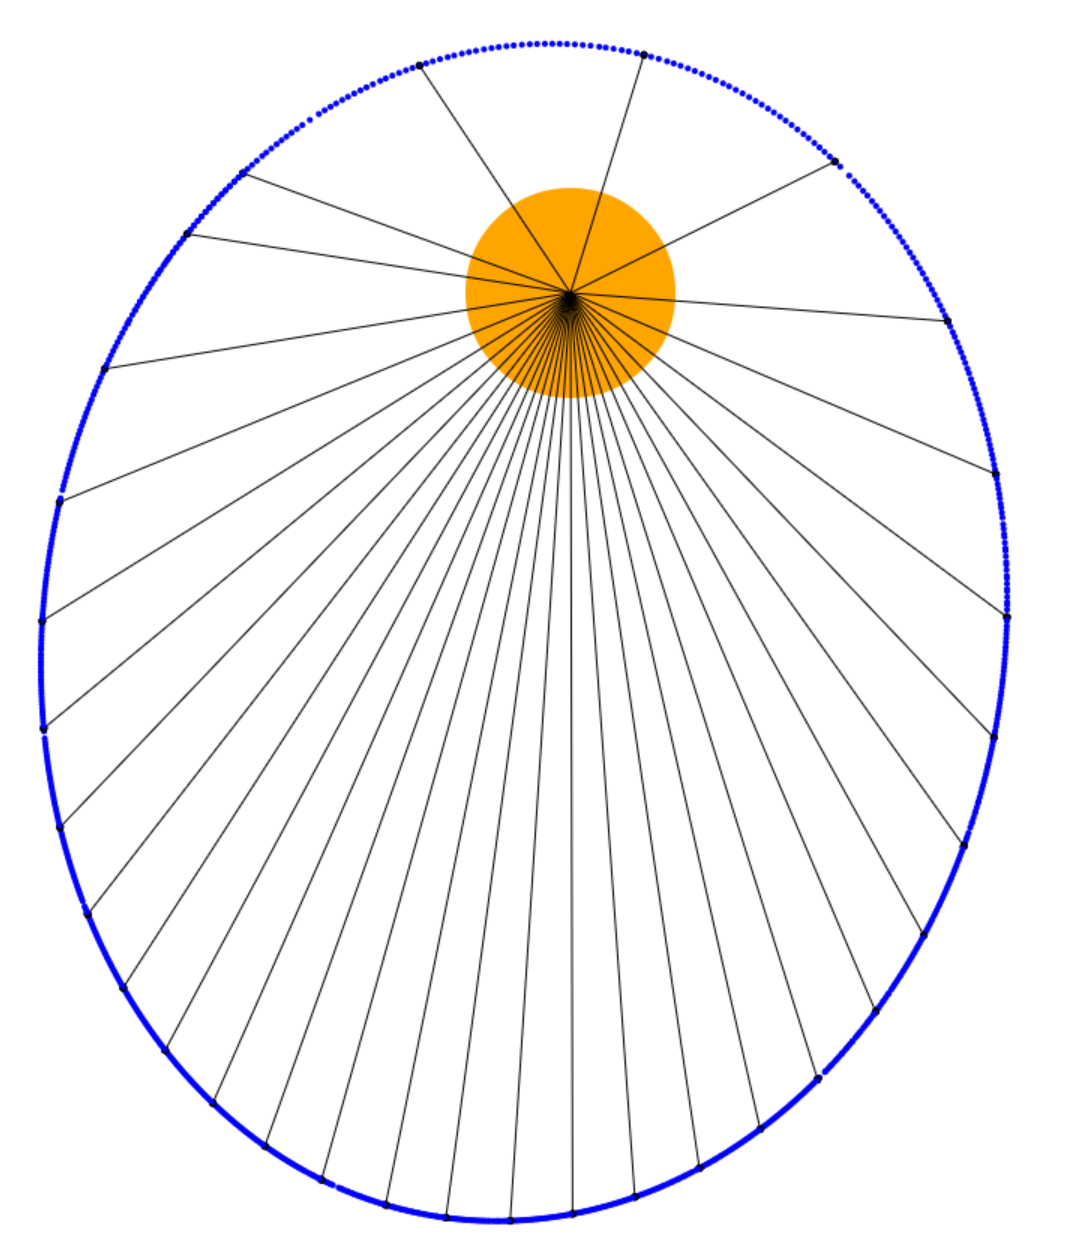
\includegraphics[width=7cm]{Figures/keplerscreenshot.png}
	\caption{Screenshot of Kepler Law test simulation}
	\label{fig:screenshot}
\end{figure}






























